%!TEX root = ../thesis.tex
%*******************************************************************************
%****************************** Third Chapter **********************************
%*******************************************************************************
\chapter{High quality assembly of a single Mosquito}

% **************************** Define Graphics Path **************************
\ifpdf
    \graphicspath{{Chapter3/Figs/Raster/}{Chapter3/Figs/PDF/}{Chapter3/Figs/}}
\else
    \graphicspath{{Chapter3/Figs/Vector/}{Chapter3/Figs/}}
\fi



\section{Background}
\par{
Exciting efforts to sequence the diversity of life are building momentum\cite{Lewin2018-lc} but one of many challenges that these efforts face is the small size of most organisms. For example, arthropods, which comprise the most diverse animal phylum, are typically small. Advances in long read sequencing over the past decade have revolutionized genome assembly and reference genome creation\cite{pacbio}\cite{oxford}, but until recently the DNA requirements for these technologies were relatively high. This made long read sequencing of single individuals impossible for many small species due to the amount of DNA that can be extracted even when consuming the whole specimen. In the standard assembly process, when considering sequences which have inexact homology, one must decide whether the differences arose from errors, haplotype differences, or paralogous sequences. If it is determined that the differences are due to heterozygosity, an assembler would collapse the sequence. However, if the assembler decides the sequences are repeats and thus represent different locations (close or distal) in the genome, they should be assembled separately (see figure \ref{figure:assembly}). As the haplotype differences increase, it reduces the assembler's ability to distinguish paralogous sequences from haplotype differences for higher divergent repeats. When one cannot distinguish these processes and no reads span the repeat (and if it is due to haplotype differences, no reads will span as the homology is highly likely to continue), the contig must end to avoid chimeric misassemblies. This results in fractious and error prone genome assemblies. One could, of course, pool multiple individuals together to meet the DNA requirements, but this has serious downsides. Using a pool of individuals increases the number of haplotypes being sequenced and increases the expected haplotype differences which reduces one's ability to distinguish paralogous sequences from haplotype variation. Moreover, the structural variation in the pool of haplotypes can cause further problems in assembly. These problems are accentuated in these small species that require pooled long read sequencing, because, while levels of heterozygosity within species vary widely across taxa, intraspecific genetic variation is often highest in small organisms\cite{Leffler2012-uh}. 
}

\begin{figure}[htbp!]

\begin{centering}
\caption{Assembly of inexact homologous sequences: heterozygosity vs paralogous sequences}\label{figure:assembly}

\sidesubfloat[]{
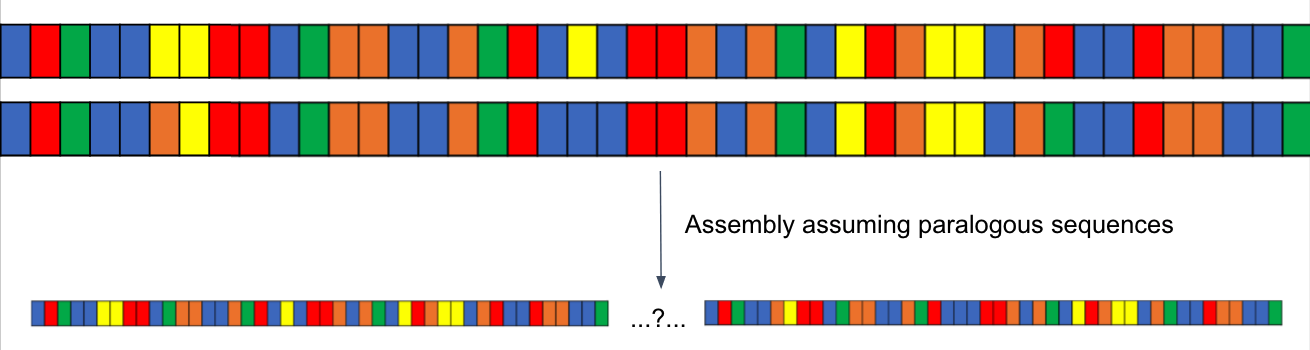
\includegraphics[width=0.95\textwidth, valign=t]{paralogues.png} \label{fig:a}
} \\
\sidesubfloat[]{
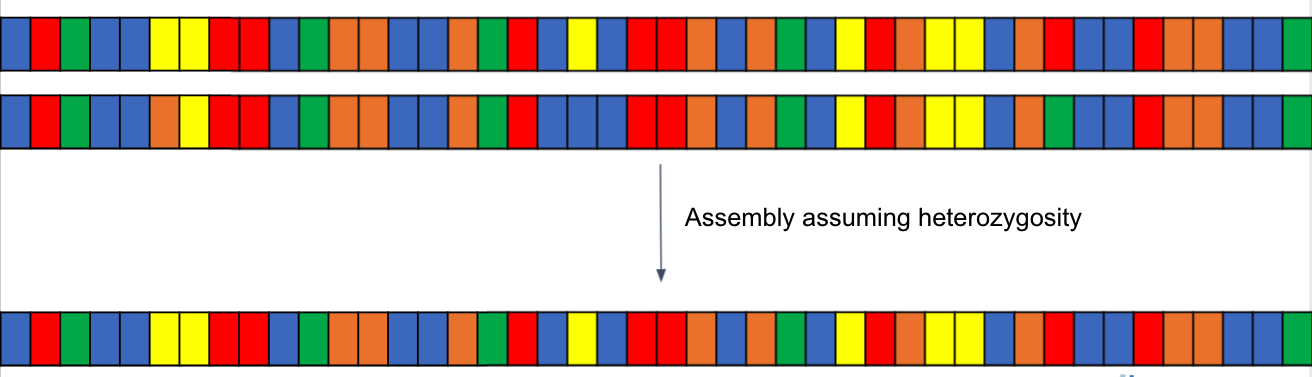
\includegraphics[width=0.95\textwidth, valign=t]{heterozygous.png} \label{fig:b}
}

\floatfoot{\small{Inexact homologous sequences and how they would be assembled if the differences are due to \textbf{a)} paralogous sequences or \textbf{b)} heterozygous differences. }}
\end{centering}
\end{figure}


\par{
To address these problems, over the past two decades, reference genomes for many small organisms have been built through considerable efforts of inbreeding organisms to reduce their heterozygosity levels such that many individuals can be pooled together for DNA extractions with more similar haplotypes. This approach has varied in its success, for example working well for organisms that are easy to inbreed (e.g., many \textit{Drosophila} species\cite{Drosophila_12_Genomes_Consortium2007-fx}), but less well for species that are difficult or impossible to inbreed (e.g., \textit{Anopheles}\cite{Neafsey2015-op}). Therefore, many efforts to sequence genomes of small organisms have relied primarily on short-read approaches due to the large amounts of DNA required for long read sequencing. For example, the recent release of 28 arthropod genomes as part of the i5K initiative used four different insert size Illumina libraries, resulting in an average contig N50 of 15 kb and scaffold N50 of 1 Mb\cite{Thomas2018-rk}.
} 

\par{
Another way to overcome DNA input requirements, while also reducing the number of haplotypes present in a DNA pool, is to limit the number of haplotypes in the pool of individuals by using offspring from a single cross. This is easier than multiple generations of inbreeding, and can be successful. For example, a recent PacBio \textit{Aedes aegypti} assembly used DNA extracted from the offspring of a single cross, thus reducing the maximum number of haplotypes for any given locus to four, thereby improving the assembly process and achieving a contig N50 of 1.3 Mb\cite{Matthews2018-th}. These four haplotypes will have recombined with each other in the cross, but recombinations are fairly rare and do not greatly increase the haplotype differences problems in assembly. Even this may run into problems though. For example, in species which mate multiple times and store sperm in a spermatheca as is the case in many diptera\cite{spermatheca}\cite{polyandry} it may be difficult to create a pure single cross. Also, these are not conducive to wild-caught organisms and must be grown in a lab for controlled crossing.
} 

\par{
However, for an initiative like the Earth BioGenome Project\cite{Lewin2018-lc} that aims to build high-quality reference genomes for more than a million described species over the next decade, generating broods to reach sufficient levels of high molecular weight DNA for long-read sequencing will be infeasible for the vast majority of organisms. Therefore, new methods that overcome the need to pool organisms are needed to support the creation of reference-quality genomes from wild-caught individuals to increase the diversity of life for which reference genomes can be assembled. Here, we present the first high-quality genome assembled with unamplified DNA from a single individual insect using a new workflow that greatly reduces input DNA requirements. Until recent advances in long read library preparation\footnote{My friend and former coworker, Brendan Galvin, was the person at PacBio who made these library preparation improvements.}\cite{mosquito_assembly}, it was not possible to obtain
enough DNA from a single individual of small organisms such as mosquitos to create a long read sequencing library from one individual. 
But for many other smaller species, this still remains the case. And it also remains the case for nanopore sequencing. 
Whether it is possible to decrease the input requirements for nanopore sequencing and to what extent are currently unknown.  
} 

\par{
In this chapter we discuss the process of making the first high quality assembly of a single mosquito and assess its quality and completeness. We first discuss the methods used for high molecular weight (HMW) DNA extraction and resulting length profiles. The extraction was done at the Sanger Institute, but the sequencing was done in California. So a further length profile is included to show the DNA length degradation from transit. We then discuss the new low input library prep and the sequencing used. We outline briefly the curation steps taken which resulted in changes to the assembly before going through each analysis in detail. Assembly quality is then assessed first through comparison of contiguity of the assembly and curated assembly against the current gold standard reference genome (Agam4 PEST). Next completeness and assembly duplication are inspected via comparing to known orthologous gene sets with BUSCO (Benchmarking Universal Single-Copy Orthologs). Finally, I do a series of genome comparisons to the PEST reference. In this, I am able to identify and correct a misassembly and uncover significant remaining duplicated haplotype assembly sequence and its cause. In this analysis, I am also able to find many improvements our assembly makes over the PEST assembly including placing of previously unplaced genes in their chromosomal context. We also dramatically reduce the assembly gaps. I found significant evidence of collapsed complex repeats in PEST that have been accurately expanded in our assembly. I then found an order-and-orientation error in the PEST reference. Finally, I show the contig coverages of the PEST reference aligned to the PacBio assembly and how much of the UNKN contigs are likely haplotigs and visually show the placement of other UNKN sequence.
} 

\par{
This work was done over two years ago now, and the field is rapidly evolving. Many of the procedures described in this chapter have become common practice and have been further improved with the advent of the HiFi data type from PacBio. Today, even higher quality genomes are being produced on a regular basis. This work represents the first, but not the last or best genome assembly of a small organism.
}

\par{
The genome we use for comparison was built using bacterial artificial chromosomes (BACs) and Sanger sequencing, the same basic technology initially used to create the human reference genome, which is highly accurate but extremely labor intensive and expensive. Our assembly allows for the use of a single individual, is relatively cheap, and is more accurate and complete than the previous gold standard \textit{Anopheles} genome. With some addition data, or by scaffolding against the PEST reference as shown in this chapter, it would also be more contiguous with fewer gaps.
}

\section{DNA Isolation}

The DNA isolation was carried out by Juliana Cudini, a fellow PhD student. \\

\par{
High molecular weight (HMW) DNA was isolated from a single \textit{Anopheles coluzzii} female from the Ngousso colony. This colony was created in 2006 from the broods of approximately 100 wild-caught pure \textit{Anopheles coluzzii} females in Cameroon (pers. comm. Anna Cohuet). Although the colony has been typically held at >100 breeding individuals, given the long time since colonization, there is undoubtedly inbreeding. A single female was ground in 200 $\mu l$ PBS using a pestle with several up and down strokes (i.e., no twisting), and DNA extraction was carried out using a Qiagen MagAttract HMW kit (PN-67653) following the manufacturer's instructions, with the following modifications: 200 $\mu l$ 1X PBS was used in lieu of Buffer ATL; PBS was mixed simultaneously with RNAse A, Proteinase K, and Buffer AL prior to tissue homogenization and incubation; incubation time was shortened to 2 h; solutions were mixed by gently flicking the tube rather than pipetting to reduce shearing and maximize extracted DNA length; and subsequent wash steps were performed for one minute. Any time DNA was transferred, wide-bore tips were used. These modifications were in accordance with recommendations from 10X Genomics HMW protocols that aim to achieve >50 kb molecules. The resulting sample contained ~250 ng of DNA, and we used the FEMTO Pulse to examine the molecular weight of the resulting DNA. This revealed a relatively sharp band at ~150 kb (figure \ref{figure:fempto2}). The DNA was shipped from the U.K. to California on cold packs, and examined again by running 500 pg on the FEMTO Pulse. While a shift in the molecular weight profile was observed as a result of transport, showing a broader DNA smear with mode of ~40 kb (figure \ref{figure:fempto}), it was still suitable for library preparation (note that this shifted profile is coincidentally similar to what is observed with the unmodified MagAttract protocol). DNA concentration was determined with a Qubit fluorometer and Qubit dsDNA HS assay kit, and 100 ng from the 250 ng total was used for library preparation.
}


\begin{figure}[htbp!]
\caption{\textit{Anopheles coluzzii} single mosquito HMW DNA extraction}
\label{figure:fempto2}
\begin{centering}
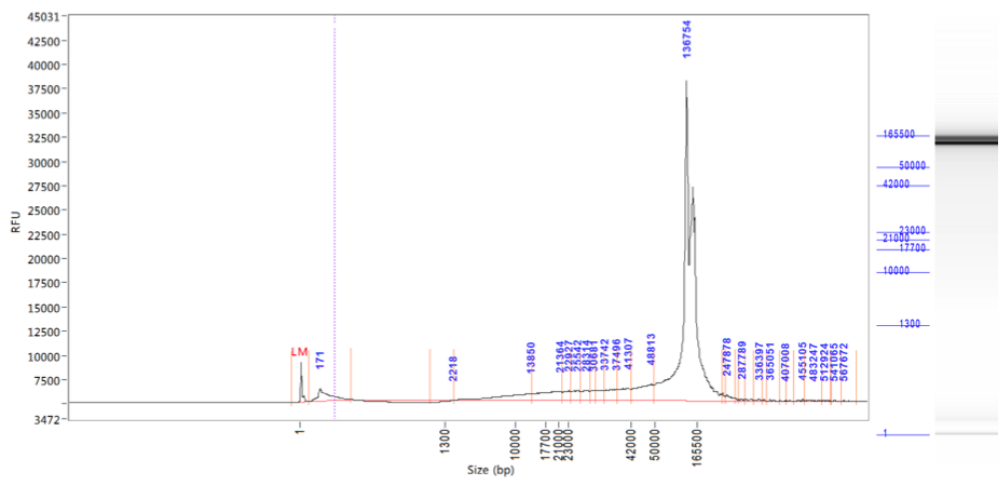
\includegraphics[width=.85\textwidth]{fempto2.png}
\floatfoot{\small{Femto Pulse evaluation of the Modified MagAttract DNA extraction prior to shipment to
California. }}
\end{centering}
\end{figure}

\section{Library prep and Sequencing}

Library prep and sequencing were performed by Sarah Kingan, Senior Scientist at PacBio. \\

\par{
A SMRTbell library was constructed using an early access version of SMRTbell Express Prep kit v2.0 from Pacific Biosciences (PacBio). Because the genomic DNA was already fragmented with the majority of DNA fragments above 20 kb (figure \ref{figure:fempto}), the sequencing library preparation protocol was modified to exclude an initial shearing step, which facilitated the use of lower input amounts, as shearing and clean up steps typically lead to loss of DNA material. After following the Express template preparation protocol, the final clean up step was simplified to just two AMPure purification steps to remove unligated adapters and very short DNA fragments. The size and concentration of the final library (figure  \ref{figure:fempto}) were assessed using the FEMTO Pulse and the Qubit Fluorometer and Qubit dsDNA HS reagents Assay kit, respectively. This resulted in a final library with a size distribution peak around 15 kb (figure \ref{figure:fempto}). 
}


\begin{figure}[htbp!]
\caption{\textit{Anopheles coluzzii} input and resulting library DNA lengths}
\label{figure:fempto}
\begin{centering}
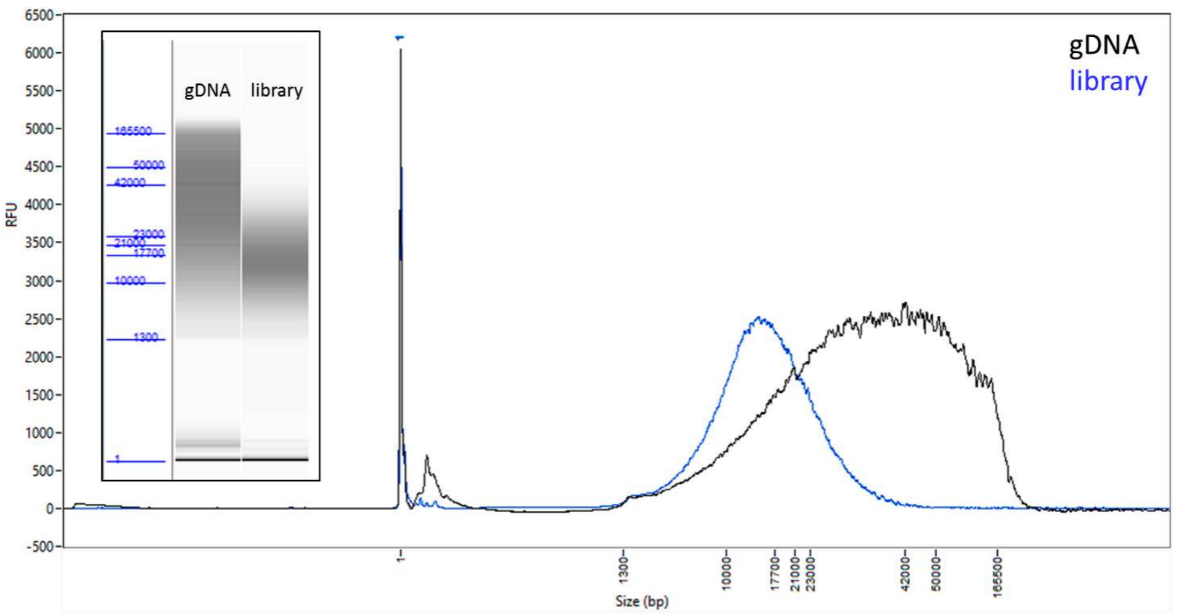
\includegraphics[width=.85\textwidth]{fempto.png}
\floatfoot{\small{FEMTO Pulse traces and gel images (inset) of the genomic DNA input (black) and the final library (blue) before sequencing. }}
\end{centering}
\end{figure}

\par{
Sequencing primer v4 and Sequel DNA Polymerase 3.0 were annealed and bound, respectively, to the SMRTbell library. The library was then sequenced on the Sequel System with Sequel Sequencing Kit 3.0. 1200 minute movie with 120 minute pre-extension and Software v6.0. A total of three SMRT cells were run generating on average 24.2 Gb of data per SMRT Cell, with average insert lengths of 8.1 kb (insert length N50 \~13 kb, table \ref{table:dataamount}). This is double the standard exposure time allowing for more data out of the same sample. However, extending exposure times has diminishing returns. The overall library yield was 59\%, which would have allowed for the sequencing of at least 8 SMRT Cells, thereby potentially allowing for genome sizes 2-3 times larger or organisms that yield 2-3 times less DNA in extraction than studied here in conjunction with this protocol.
}

\begin{table}[htbp!]
\caption{Run statistics for Sequel SMRT Cells.}\label{table:dataamount}
\begin{tabular}{| c | c | c | c | c | c |}
\hline
Loading & Gb/cell & Mean  & N50 &  Mean &  N50  \\
concentration & & Polymerase & Polymerase & Subread & Subread \\
& & Read & Read & Length & Length \\ 
& & Length &Length & & \\\hline
5 pM & 24.1 & 40290 & 116615 & 8185 & 12978 \\\hline
5 pM & 23.6 & 40077 & 114807 & 8254 & 13132 \\\hline
6 pM & 25.0 & 47177 & 122898 & 8012 & 12751 \\\hline
\end{tabular}
\end{table}



\section{Assembly}

The assembly was run by Sarah Kingan, Senior Scientist at PacBio. My main role was in quality assessment and comparative genomics. \\

\par{
The genome was assembled using FALCON-Unzip, a diploid assembler that captures haplotype variation in the sample\cite{falcon}. A single subread per zero-mode waveguide (ZMW) was used for a total of 12.8 Gb of sequence from three SMRT Cells, or ~48-fold coverage of the ~266 Mb genome. Subreads longer than 4559 bp were designated as seed reads and used as template sequences for preassembly/error correction. A total of 8.1 Gb of preassembled reads was generated (~30-fold coverage). After assembly and haplotype separation by FALCON-Unzip, two rounds of polishing were performed to increase the consensus sequence quality of the assembly, aligning the PacBio data to the contigs and computing consensus using the Arrow consensus caller\cite{arrow}. The first round of polishing was part of the FALCON-Unzip workflow and used a single read per ZMW that was assigned to a haplotype. The second round of polishing was performed in SMRT Link v 6.0.0.43878, concatenating primary contigs and haplotigs into a single reference and aligning all subreads longer than 1000 bp (including multiple subreads from a single sequence read, mean coverage 184-fold) before performing genomic consensus calling. The alignments (BAM files) produced during the two rounds of polishing were used to assess confidence in the contig assembly in regions with rearrangements relative to the AgamP4 PEST assembly for \textit{Anopheles gambiae} (GenBank assembly accession GCA\_000005575.2)\cite{PEST}\cite{PEST2}. We referred to the first round of polishing as using unique subreads and the second round as using all subreads.
} 

\par{
We explored the performance as a function of the number of SMRT Cells used for the assembly (table \ref{table:smrtcells}), and found that while a single SMRT Cell was insufficient to result in high-quality assembly, data from two or three SMRT Cells generated a highly contiguous assembly of the correct genome size. We proceeded with the three-cell assembly for all subsequent analyses because it gave the most contiguous and complete assembly results.
}

\begin{table}[htbp!]
\caption{Assembly quality vs the amount of data used.}\label{table:smrtcells}
\begin{tabular}{| c | c | c | c |}
\hline
 & \textbf{1 SMRT cell} & \textbf{2 SMRT cells} & \textbf{3 SMRT cells} \\\hline
 \textbf{Total bases (Gb)} & 23.6 & 48.5 & 72.7 \\\hline
  \textbf{Total unique bases (Gb)} & 4.46 & 8.31 & 12.8 \\\hline 
  \textbf{Unique coverage} & 17x & 31x & 45x \\\hline 
  \textbf{Assembly size (Mb)} & 150 & 265 & 271 \\\hline 
  \textbf{Number of contigs} & 3,290 & 815 & 580 \\\hline 
  \textbf{Contig N50 (Mb)} & 0.066 & 1.5 & 3.5 \\\hline
\end{tabular}
\floatfoot{\small{Statistics for \textit{Anopheles coluzzii} de novo genome assemblies as a function of the number of
SMRT Cells used for the assembly. One cell failed to assembly the whole genome. Two and three cells assembled the majority of the genome but quality improved with 3 cells.}}
\end{table}
%The resulting primary assembly consisted of 372 contigs totaling 266 Mb in length, with a contig N50 of 3.5 Mb and a secondary 
%haplotype assembly totalling 78.5 Mb. \ref{table:assemblydata} shows various assembly statistics of the long read assembly and the current 
%reference assembly of the closely related \textit{Anopheles gambiae}\cite{PEST}\cite{PESTupdate}\cite{PESTchromitin}\cite{gambiaeref}. 




\section{Curation}

\par{
The contigs were screened by the Sanger Institute and NCBI to identify contaminants and mitochondrial sequence\cite{sangercuration}. Windowmasker was used to mask repeats and the MegaBLAST algorithm was run (with parameter settings: -task megablast -word\_size 28 -best\_hit\_overhang 0.1 -best\_hit\_score\_edge 0.1 -dust yes -evalue 0.0001 -min\_raw\_gapped\_score 100 -penalty 5 -perc\_identity 98.0 -soft\_masking true -outfmt 7) on the masked genome versus all complete bacterial genomes to find hits with  greater than 98\% homology\cite{windowmasker}\cite{megablast}. One contig (\#20) was identified as a complete 4.24 Mb bacterial genome, closely related to \textit{Elizabethkingia anophelis}, which is a common gut microbe in Anopheles mosquitoes\cite{kingia}\cite{blobtoolkit}. It was separated from the mosquito assembly and submitted to NCBI separately. We also identified two contigs of mitochondrial origin that each contained multiple copies of the circular chromosome. Full length copies of the mitochondrial chromosome in the higher quality contig differed by only a single base and the consensus sequence was reported as the mitochondrial genome. One of these copies was discarded.
} 

\par{
In addition, I screened the primary assembly for duplicate haplotypes using Purge Haplotigs\cite{purge} with default parameters and coverage thresholds of 20, 150, and 700. While FALCON-Unzip resolved haplotypes over ~30\% of the genome, 110 genes appeared as duplicated copies in the BUSCO analysis, indicating that highly divergent haplotypes may be assembled as distinct primary contigs as has been observed in other mosquito genome assemblies\cite{aegypti}\cite{funestus}. The presence of duplicated haplotypes can result in erroneously low mapping qualities in resequencing studies and cause problems in downstream scaffolding. Using the Purge Haplotigs software\cite{purge}, I identified 165 primary contigs totalling 10.6 Mb as likely alternate haplotypes, although there remains a possibility that some may be repeats. These contigs were transferred to the alternate haplotig set.
} 


\par{
In the process of comparing the assembly to the PEST reference (described later), I found one large potential heterozygous interchromosomal rearrangement between 2L and 3R (see figure \ref{figure:misassembly}). Upon further exploration, this was not supported by any subreads mapping across the breakpoint (figure \ref{figure:misassembly}). The putative breakpoints were identified by aligning the PacBio contigs to PEST with minimap2 (asm5 setting)\cite{minimap2}, and the start and end position of each aligned subread was determined using bedtools bamtobed\cite{bedtools}. This 4.9 Mb contig had no reads spanning the putative breakpoint when either unique or all subread alignments were examined and thus I designated this a chimeric misassembly, and split the contig into two.
}



\section{Assembly quality assessment}


\par{
Using the FALCON-Unzip assembler\cite{falcon}, the resulting primary de novo assembly consisted of 372 contigs totaling 266 Mb in length, with half of the assembly in contigs (contig N50) of 3.5 Mb or longer (table \ref{table:assemblydata}). FALCON-Unzip also generated 665 alternate haplotigs, representing regions of sufficient heterozygosity to allow for the separation of the maternal and paternal haplotypes. These additional phased haplotype sequences spanned a total of 78.5 Mb (i.e., 29\% of the total genome size was separated into haplotypes), with a contig N50 of 223 kb (table \ref{table:assemblydata}). 
}


\begin{table}[htbp!]
\caption{Assembly statistics}\label{table:assemblydata}
\begin{center}
\begin{tabular}{ | l | l | l | l | l |}
\hline
\multicolumn{2}{|c|}{} & \textbf{Initial} & \textbf{Curated} & \textbf{PEST} \\
\multicolumn{2}{|c|}{} & \textbf{Assembly} & \textbf{Assembly} & \textbf{reference} \\
\hline
\multirow{3}{5em}{\textbf{Primary Assembly}}
& Size (Mb) & 266 & 251 & 224 \\
\cline{2-5}
& Number Contigs & 372 & 206 & 27,063 \\
\cline{2-5}
& Contig N50 (Mb) & 3.52	& 3.47	& 0.025 \\
\hline%\cline{2-5}
\multirow{3}{5em}{\textbf{Alternate Haplotigs}}
& Size (Mb) & 78.5 & 	89.2	& unresolved \\
\cline{2-5}
& Number Contigs & 665 &	830& 	N/A \\
\cline{2-5}
& Contig N50 (Mb) & 0.22	& 0.199	& N/A \\
\hline
\end{tabular}
\end{center}
\end{table}




\subsection{BUSCO analysis: completeness and duplication/haplotig retainment}

\par{
To evaluate genome completeness and sequence accuracy of the currated assembly, we performed alignment analyses to a set of conserved genes. Using the diptera set of the BUSCO (Benchmarking Universal Single-Copy Orthologs) gene collection, we observed 98\% of the ~2800 genes were complete and >95\% occurred as single copies (table \ref{table:busco}). By comparison, the previous assembly had 87.5\% complete BUSCO alignments, indicating that a fraction of the genome was missing in that assembly. The percentage of duplicated genes was reduced from 3.9\% to 2.4\% after curation.  Additional analyses are required to distinguish true gene duplication events from incomplete purging of duplicated haplotypes (see discussion below and figure \ref{figure:haplotig}). In addition, we evaluated assembly completeness against a curated set of genes (AgamP4.10 gene set) from the \textit{Anopheles gambiae} PEST reference, using a previously described script\cite{avian}. We aligned to the primary assembly a closely related species gene set (the most recent \textit{Anopheles gambiae} (AgamP4.10) gene set), resulting in 14,972 alignments (99.5\%) and an average alignment length of 96.6\%, and with >96\% of alignments showing no frame shift-inducing indels.
}


\begin{table}[htbp!]
\caption{BUSCO analysis.}\label{table:busco}
\begin{tabular}{| c | c | c | c |}
\hline
 \textbf{Gene count (\%)} & \textbf{Initial} & \textbf{Curated} & \textbf{PEST} \\\hline
   & \textbf{Assembly} & \textbf{Assembly} & \textbf{Reference} \\\hline
 \textbf{Complete} & 2745 (98.0) & 2747 (98.1) & 2448 (87.5) \\\hline
  \textbf{Complete Single Copy} & 2635 (94.1) & 2680 (95.7) & 2446 (87.4)  \\\hline 
  \textbf{Complete Duplicated} & 110 (3.9) & 67 (2.4) & 3 (0.1) \\\hline 
  \textbf{Fragmented} & 25 (0.9) & 25 (0.9) & 190 (6.8) \\\hline 
  \textbf{Missing} & 29 (1.1) & 28 (1.0) & 160 (5.7) \\\hline 
   \textbf{Total} & 2799 (100) & 2799 (100) & 2799 (100) \\\hline
  
\end{tabular}
\floatfoot{\small{Analysis of single copy conserved genes using BUSCO v3.0.2 and the diptera gene set. Initial assembly: primary contigs from the 3-cell de novo FALCON-Unzip assembly. Curated assembly: Primary contigs after removal of bacterial contaminants and duplicated haplotypes. Previous reference from\cite{PEST}
GCA\_000150765.1.}}
\end{table}



%According to Busco \cite{busco} analysis of the primary assembly, 110 genes were duplicated indicating some resolved heterozygosity (haplotigs) remaining in the primary assembly. 
%The presence of duplicated haplotypes in a reference genome can result in erroneously low mapping qualities in resequencing studies and cause problems when scaffolding. 
%We used the Purge Haplotigs software \cite{purge} and identified 165 primary contigs totalling 10.6 Mb as likely haplotigs which were then moved to the alternate haplotigs fasta.

%There are many problems with the current \textit{Anopheles gambiae} reference including 6302 gaps of Ns in the 
%primary chromosome scaffolds ranging from 20 bases to 36 kb and 55 gaps of 10 kb that the AGP (A Golden Path) file on Vectorbase annotates as ``contig'' endings. 
%This reference also contains a large bin of unplaced contigs (27.3 Mb excluding Ns) designated as the ``UNKN'' (unknown) chromosome. 
%However, it is the previously best characterized \textit{Anopheles} assembly which should be very closely related to the \textit{coluzzii} species so 
%we endeavored to make comparisons between them. We aligned the assembly contigs to the reference with minimap2 
%and then attempted to assign contigs to chromosomes as well as order and orient them. The new assembly is highly concordant with the reference over the entire 
%genome, allowing the placement of the long PacBio contigs into chromosomal contexts (figure \ref{figure:dotplot}). We also showed that the assembly 
%correctly expanded long repeats that had been collapsed in the reference (figure \ref{figure:repeat}) and that the assembly resolved an incorrect 
%order and orientation of the scaffolding of chromosome X (figure \ref{figure:x_inversion}).





\subsection{Comparison to \textit{Anopheles gambiae} PEST reference}

\par{
The \textit{Anopheles gambiae} genome, published in 2002, was created using BACs and Sanger sequencing\cite{PEST}. Further work over the years to order and orient contigs improved this reference\cite{PEST2}\cite{heterochromatin} and to date, AgamP4 (https://vectorbase.org/organisms/anopheles-gambiae/pest/agamp4) remains the highest quality Anopheles genome among the 21 that have now been sequenced\cite{16anopheles}. However, there are many problems with this reference genome. AgamP4 PEST still has 6302 gaps of Ns in the primary chromosome scaffolds ranging from 20 bases to 36 kb, including 55 gaps of 10 kb that the AGP (A Golden Path) file on Vectorbase annotates as contig endings. The AgamP4 genome was generated from a lab strain known as PEST (Pink Eye STandard) that is long deceased and also was an accidental mixture of two incipient species, previously known as `M' and `S'. To address this, the genomes of pure `M' and `S' from new colonies established in Mali were sequenced using only Sanger sequencing\cite{anophdivergence}. Since then, the `S' form has retained the name \textit{Anopheles gambiae} sensu stricto, and the `M' form has acquired species status and a new name, \textit{Anopheles coluzzii}\cite{gambiaecomplex}. It is important to note that while these species show assortative mating, they can hybridize in nature and their hybrids are fully fertile and viable\cite{assortativemating}. Given this fact, and the fact that both pure species assemblies remain highly fragmented, I compared our assembly to the best available \textit{Anopheles gambiae} genome (i.e., AgamP4 PEST) to evaluate contiguity and to help order and orient the contigs.
} 

\par{
To assess the quality of contig assembly and concordance with existing assemblies, the curated primary contigs were aligned to the PEST \textit{Anopheles gambiae} reference genome \cite{PEST}\cite{PEST2} using minimap2 with the map-pb settings\cite{minimap2}. For the purpose of comparison, contigs were ordered and oriented according to their median alignment position and majority alignment orientation on the chromosome to which they had the most aligned bases. A python script was used in conjunction with ggplot using geom\_segments to generate alignment plots. This software is an alternative to the commonly used nucmer/mummer\cite{mummer} and is available at \href{https://github.com/wheaton5/assembly\_comparison\_scripts}. One important difference is that these only show the single best alignment for a given span of contig sequence and is not a dotplot which would show all similar sequences above some threshold.
} 

\par{
The new PacBio assembly is highly concordant with the AgamP4 PEST reference over the entire genome, allowing the placement of the long PacBio contigs into chromosomal contexts (see figure \ref{figure:dotplot}). In addition, the high contiguity of the PacBio contigs allows for the resolution of many gaps in the chromosomal PEST contigs. Note that the only gaps in the PacBio assembly are at contig ends, whereas there are many gaps in PEST that are not annotated as contig breaks so the percent Ns per megabase of PEST is overlaid in the graphs in figure \ref{figure:dotplot}. 
}

\begin{figure}[htbp!]

\caption{Comparison of the assembly with the PEST reference}
\label{figure:dotplot}
\begin{centering}
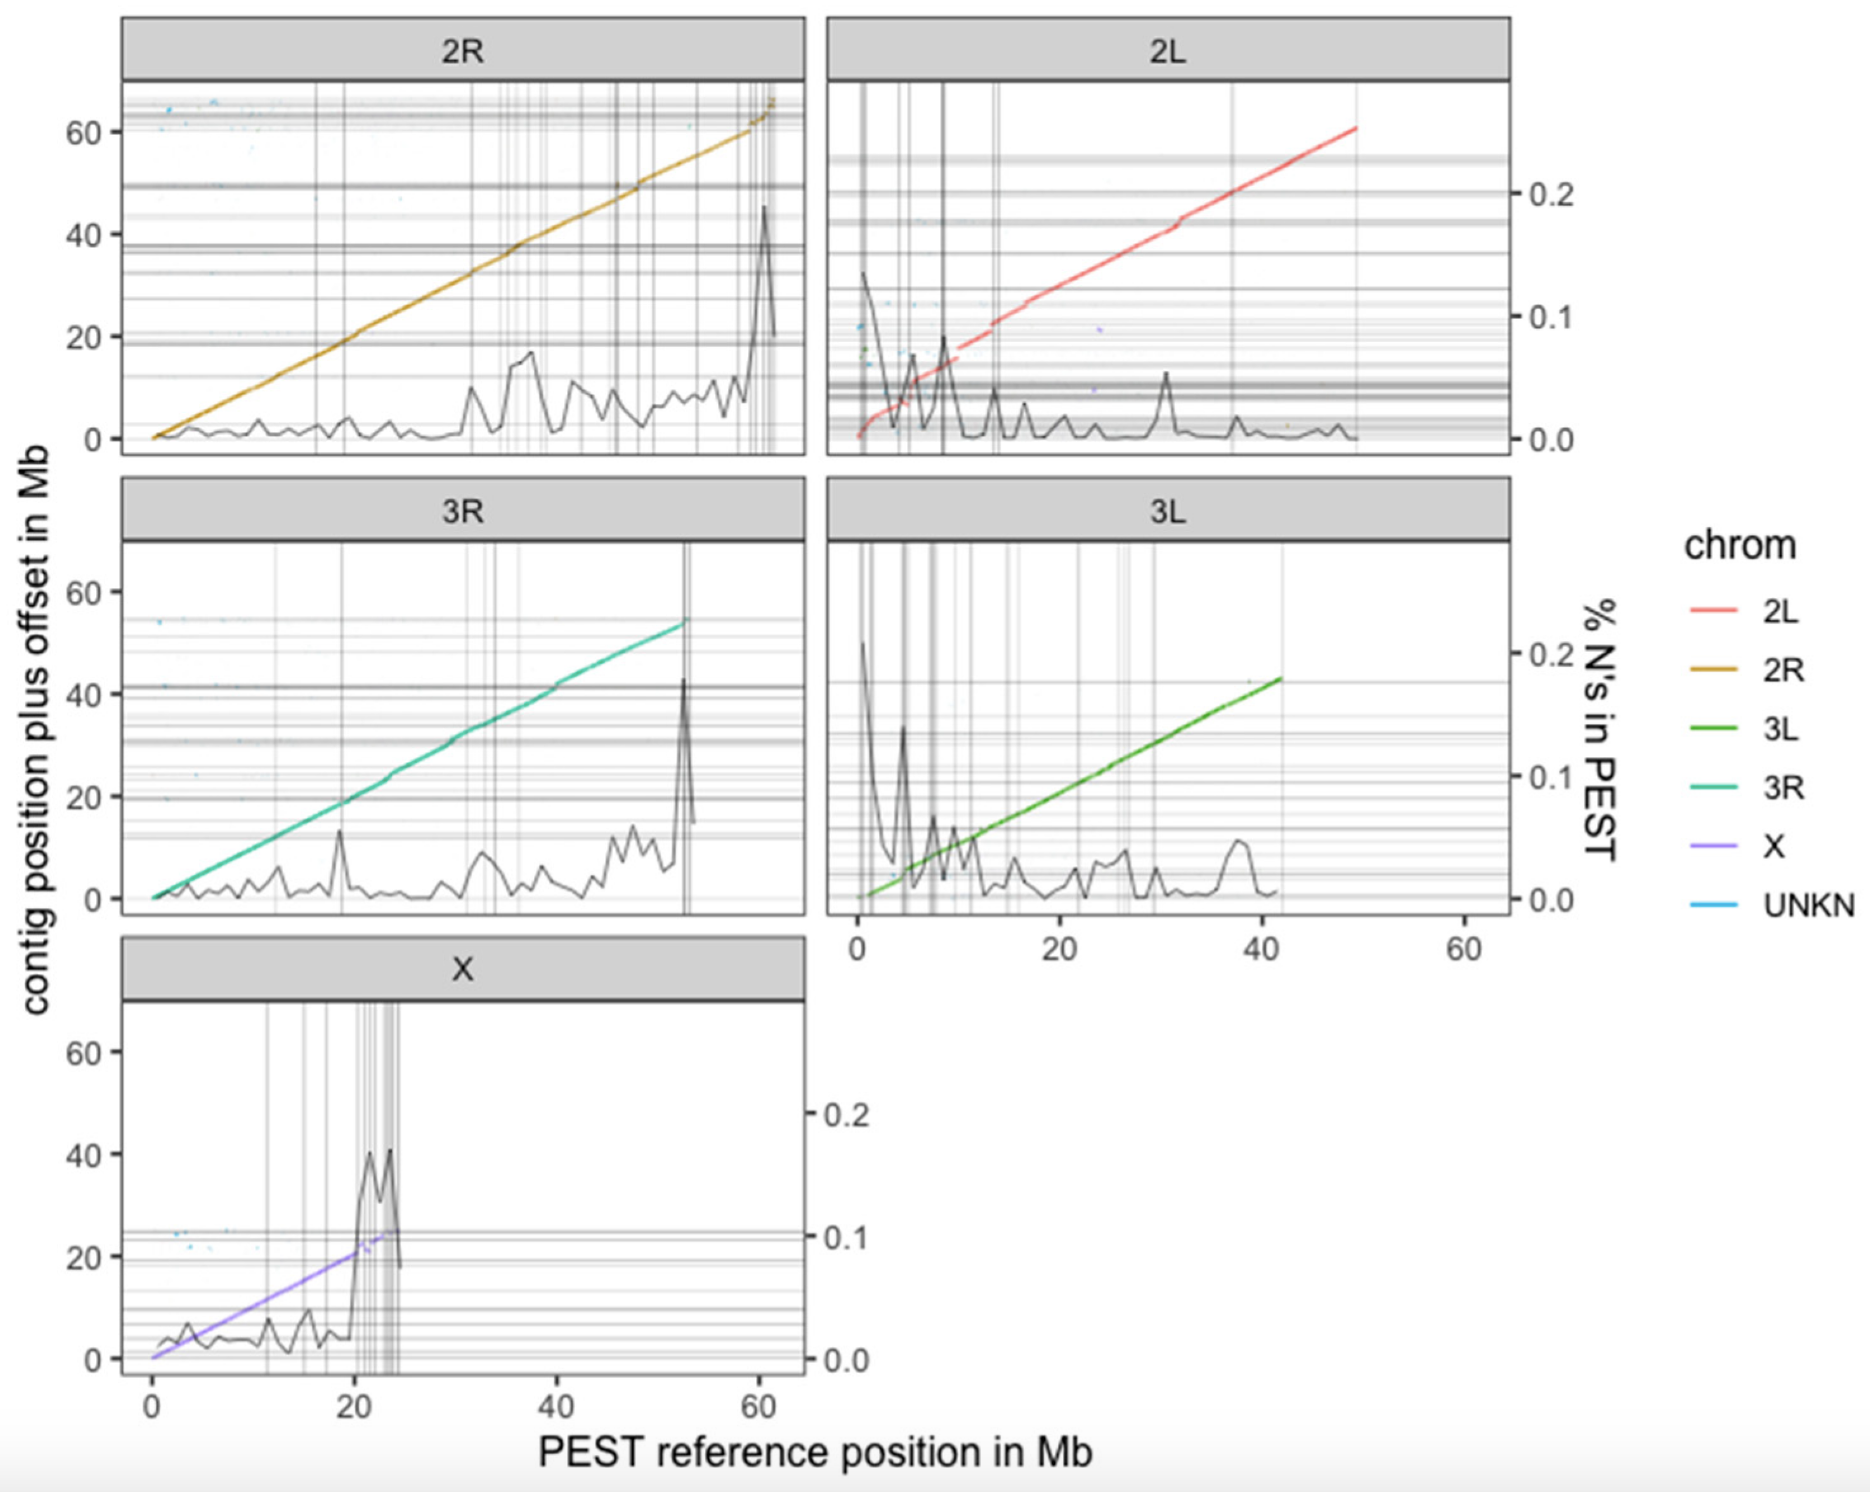
\includegraphics[width=1.0\textwidth]{dotplot.png}
\floatfoot{\small{Alignment of the curated PacBio contigs to the AgamP4 PEST reference. Alignments are colored by the primary PEST reference chromosome to which they align but are placed in the panel and Y offset to which the contig as a whole aligns best. Contig ends are denoted by horizontal lines in the assembly and vertical lines in PEST. However, there are many Ns in PEST not annotated as contig breaks so the percent Ns per megabase of PEST is overlaid (scale on the right Y axis). There are no Ns in the PacBio assembly, but there may be gaps between the PacBio assembly contigs.}}
\end{centering}
\end{figure}


\subsection{Identification and correction of misassembly}

\par{
Large regions (>200 kb) of discordant alignment of the contigs to the PEST reference where inspected further. Discordant alignments were categorized into one of three cases. 1. Large portions of a single contig aligned discordantly (e.g., to multiple PEST reference chromosomes). 2. Large regions in PEST where multiple assembly contigs aligned to the same reference region.  3. Large region in PEST where assembly contigs did not align. 
} 
\par{
First, I considered discordant alignments where large portions of a single contig aligned in very different locations of the PEST reference. Using the alignment plots as described above, I colored each alignment by that contig's primary chromosome. Immediately one cross-chromosome contig alignment stuck out (see figure \ref{figure:misassembly}). I then evaluated the evidence for the assembly join at this breakpoint by aligning the subreads to the assembly and inspected the breakpoint region in IGV (figure \ref{figure:misassembly}). I found a repeat sequence that reads from each end would align into, but found no reads that spanned the repeat. This indicated to us that this was a chimeric misassembly, and I split the contig into two.
} 
\par{
I also noted many smaller cross-chromosome alignments between contigs which primarily aligned to one of the five of PEST's chromosom-arm scaffolds and the UNKN (unknown) scaffold (not a true scaffold, just a collection of unplaced contigs). This is discussed further in section \ref{section:unkn} by using these alignments to place genes and other genomic sequence in its proper chromosomal context which were previously unplaced.
}

\begin{figure}[htbp!]
\caption{Chimeric assembly}
\label{figure:misassembly}
\begin{centering}
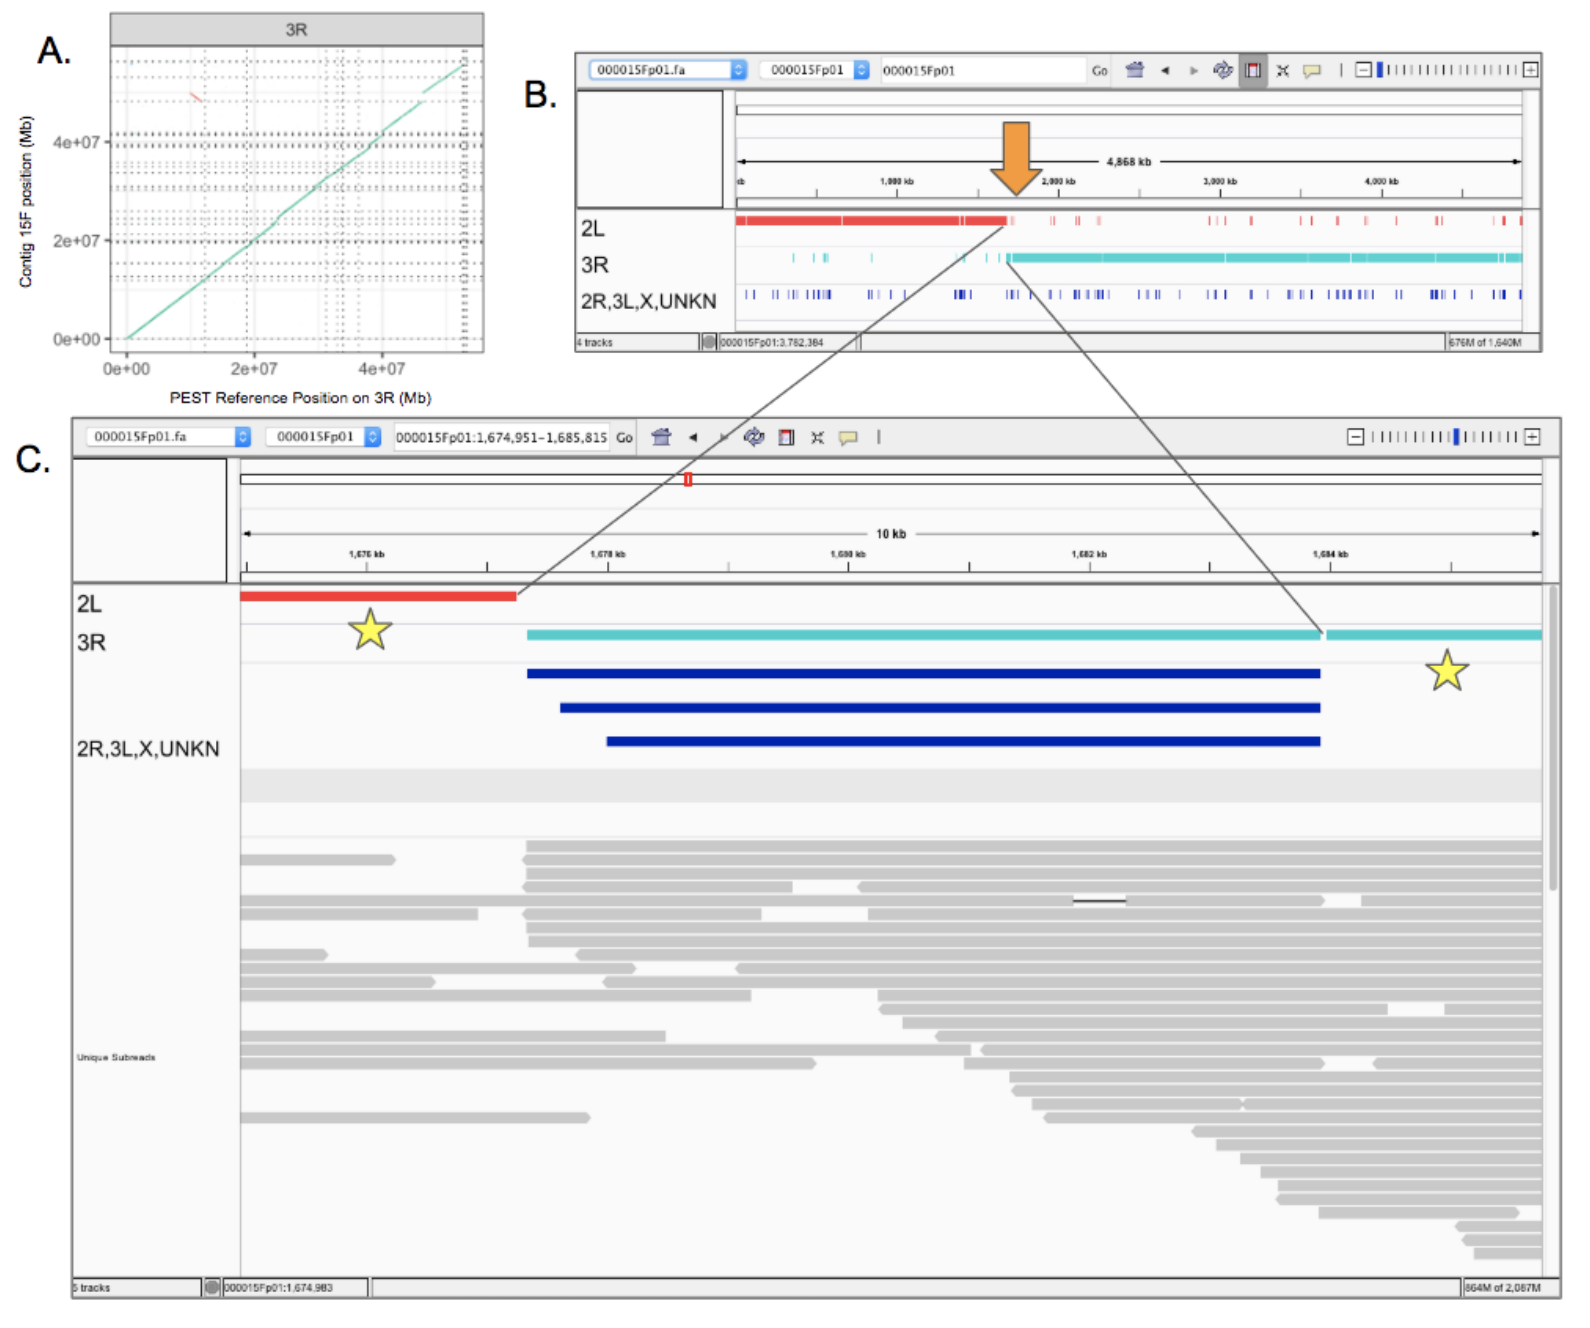
\includegraphics[width=1.0\textwidth]{misassembly.png}
\floatfoot{\small{A chimeric contig between 2L and 3R. A. Alignment of PacBio contigs to PEST identifies a candidate chromosomal rearrangement. B. IGV screenshot of breakpoint (orange arrow) localized by alignment of contig to PEST. Red: alignment to 2L, turquoise: alignments to 3R, navy blue: alignments to other chromosomes and unplaced contigs. C. IGV visualization of mapped unique subreads at breakpoint shows 0 subreads mapping across the central repetitive region into the unique flanking sequence on the left (2L) and right (3R) (stars). A count of spanning reads was also determined with bedtools bamtobed utility. The 6.5kb central region aligns to four loci in the PEST genome and has ~370 bp of sequence similarity to the Tc1-like transposase gene in \textit{Anopheles gambiae}.}}
\end{centering}
\end{figure}

\subsection{Remaining haplotig sequence on ends of contigs}

\par{
Next, large discordant regions where multiple contigs align to the same region in PEST were identified and evaluated. I found these regions by running samtools depth on the contig-PEST alignments, compressing to a bed file of contiguous regions of the same coverage, and then plotting to visually see where large sections are discordant (see figure \ref{figure:haplotig}). Using this, I found several very large segments of coverage two. Further inspection was done by zooming in to those regions specifically in the alignment plots. I observed that ends of contigs were aligned to the same position in the PEST genome. I then mapped the subreads to the assembly and assessed coverage in these regions. As expected if these were haplotig regions, the coverage was roughly half in the overlapping alignment regions. This clearly revealed that contigs were assembling the two haplotypes separately and were not removed by purge haplotigs. This is because purge haplotigs looks for contigs which are fully contained by another contig and it keeps the longer contig and removes the shorter haplotig. This results in regions where the assembly has assembled both haplotypes separately but one contig does not fully contain the other contig, the haplotig sequence remains (see figure \ref{figure:haplotig}). This realization spawned another project in our lab to improve haplotig purging by combining coverage of reads mapped to the assembly with sequence similarity to identify and remove haplotig sequence even when not fully contained by another contig\cite{purgedups} improving on the two previously available methods\cite{purge}\cite{haplomerger}.
}


\begin{figure}[htbp!]

\caption{Evidence of remaining haplotig contig ends.}

\label{figure:haplotig}
\begin{centering}
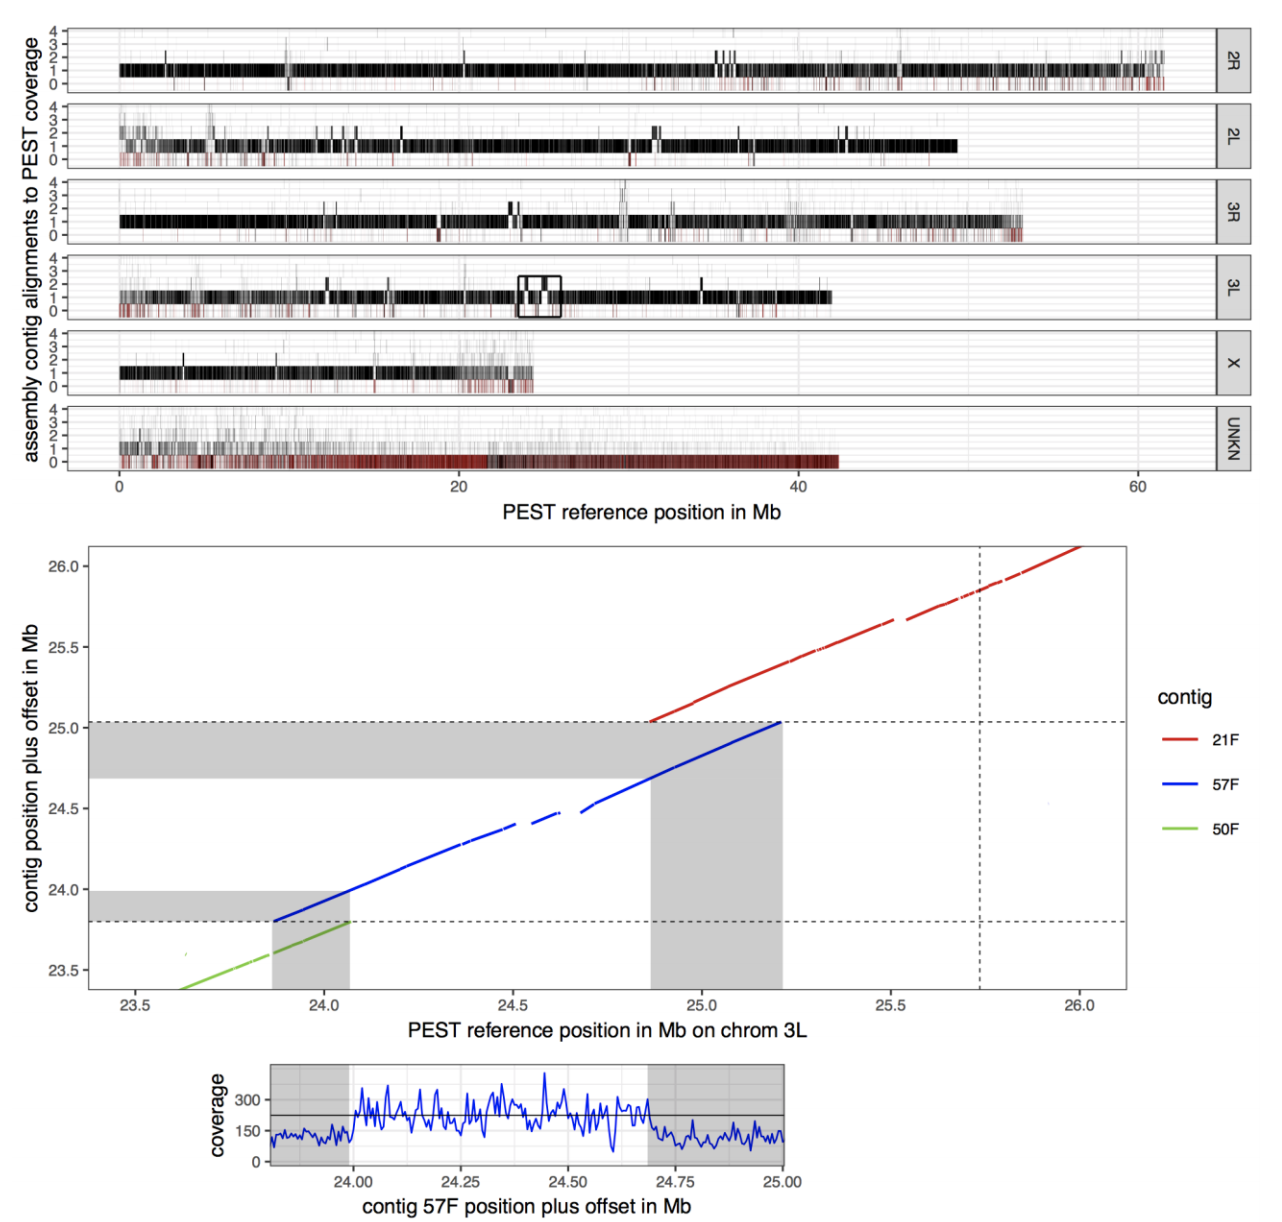
\includegraphics[width=\textwidth]{haplotigity.png}
\floatfoot{\small{Alignment and coverage plot (top) of the PacBio assembly contigs relative to PEST,
and magnification of one area of excess coverage (bottom). In the top panel, the number of
alignments of PacBio contigs to PEST are represented by black bars, with most of the genome
showing a 1:1 correspondence to PEST. Red denotes Ns in the reference. Isolated areas of
higher number of contig alignments are visible, one of which (black box) is magnified in the
bottom panel. Here, the ends of neighboring contigs overlap, which is currently not resolved with
the Purge Haplotigs software since the overlap is only partial. The sequencing depth of PacBio
reads for the central (blue) contig (57F) corroborate this interpretation, exhibiting half of the
expected coverage in the greyed regions of contig overlap, and with the corresponding ends of
the red and green contigs complementing with the other half of coverage, respectively (not
shown for clarity).}}
\end{centering}
\end{figure}

\par{
And finally, I considered large discordant regions in which no assembly contigs align to the PEST reference. In general this is rare in the chromosomal scaffolds. Most of the zero contig-coverage areas of the contig on PEST alignment file are location in which the PEST contains Ns. And the large majority of zero contig coverage areas are in the UNKN scaffold. I explored the largest of the zero contig coverage region in the chromosomal PEST scaffolds (figure \ref{figure:nocovplot}). I saw that this region is flanked by sections of Ns and that very few PacBio subreads map to the non N regions between indicating that this sequence may be low quality, possible derived from contamination, or be a biological difference (large insertion in PEST) between the two species.
}

\begin{figure}[htbp!]

\caption{No contig coverage region}
\label{figure:nocovplot}
\begin{centering}
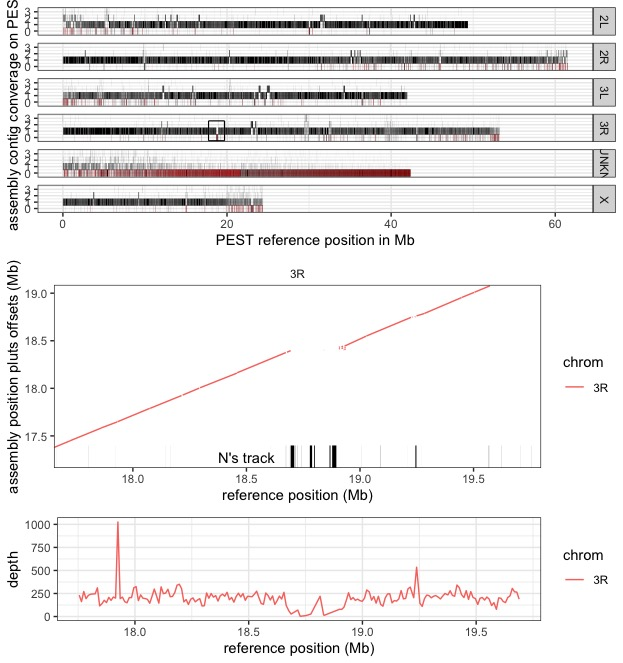
\includegraphics[width=1.0\textwidth]{Nocovplot.jpeg}
\floatfoot{\small{ Top: outlines large region with zero coverage in chromosomal scaffold 3R on PEST reference. Middle: Zoom in of alignment plot in that region with Ns track showing regions of Ns flanking this sequence with another section of Ns in the middle. Bottom: shows subread depth when aligned to the PEST reference showing decreased mapping in this region.}}
\end{centering}
\end{figure}



\subsection{Expansion of previously collapsed repeat}

\par{
The new PacBio assembly makes many improvements when compared to the PEST assembly. For example, a single contig from the new PacBio assembly expanded a tandem repeat region on chromosome 2L that in PEST was collapsed, while also filling in many Ns (gaps) in PEST, and also spanning a break between PEST scaffolds set to 10,000 Ns (see figure \ref{figure:repeat}).
}

\begin{figure}[htbp!]

\caption{Example of expansion of previously collapsed repeat}
\label{figure:repeat}
\begin{centering}
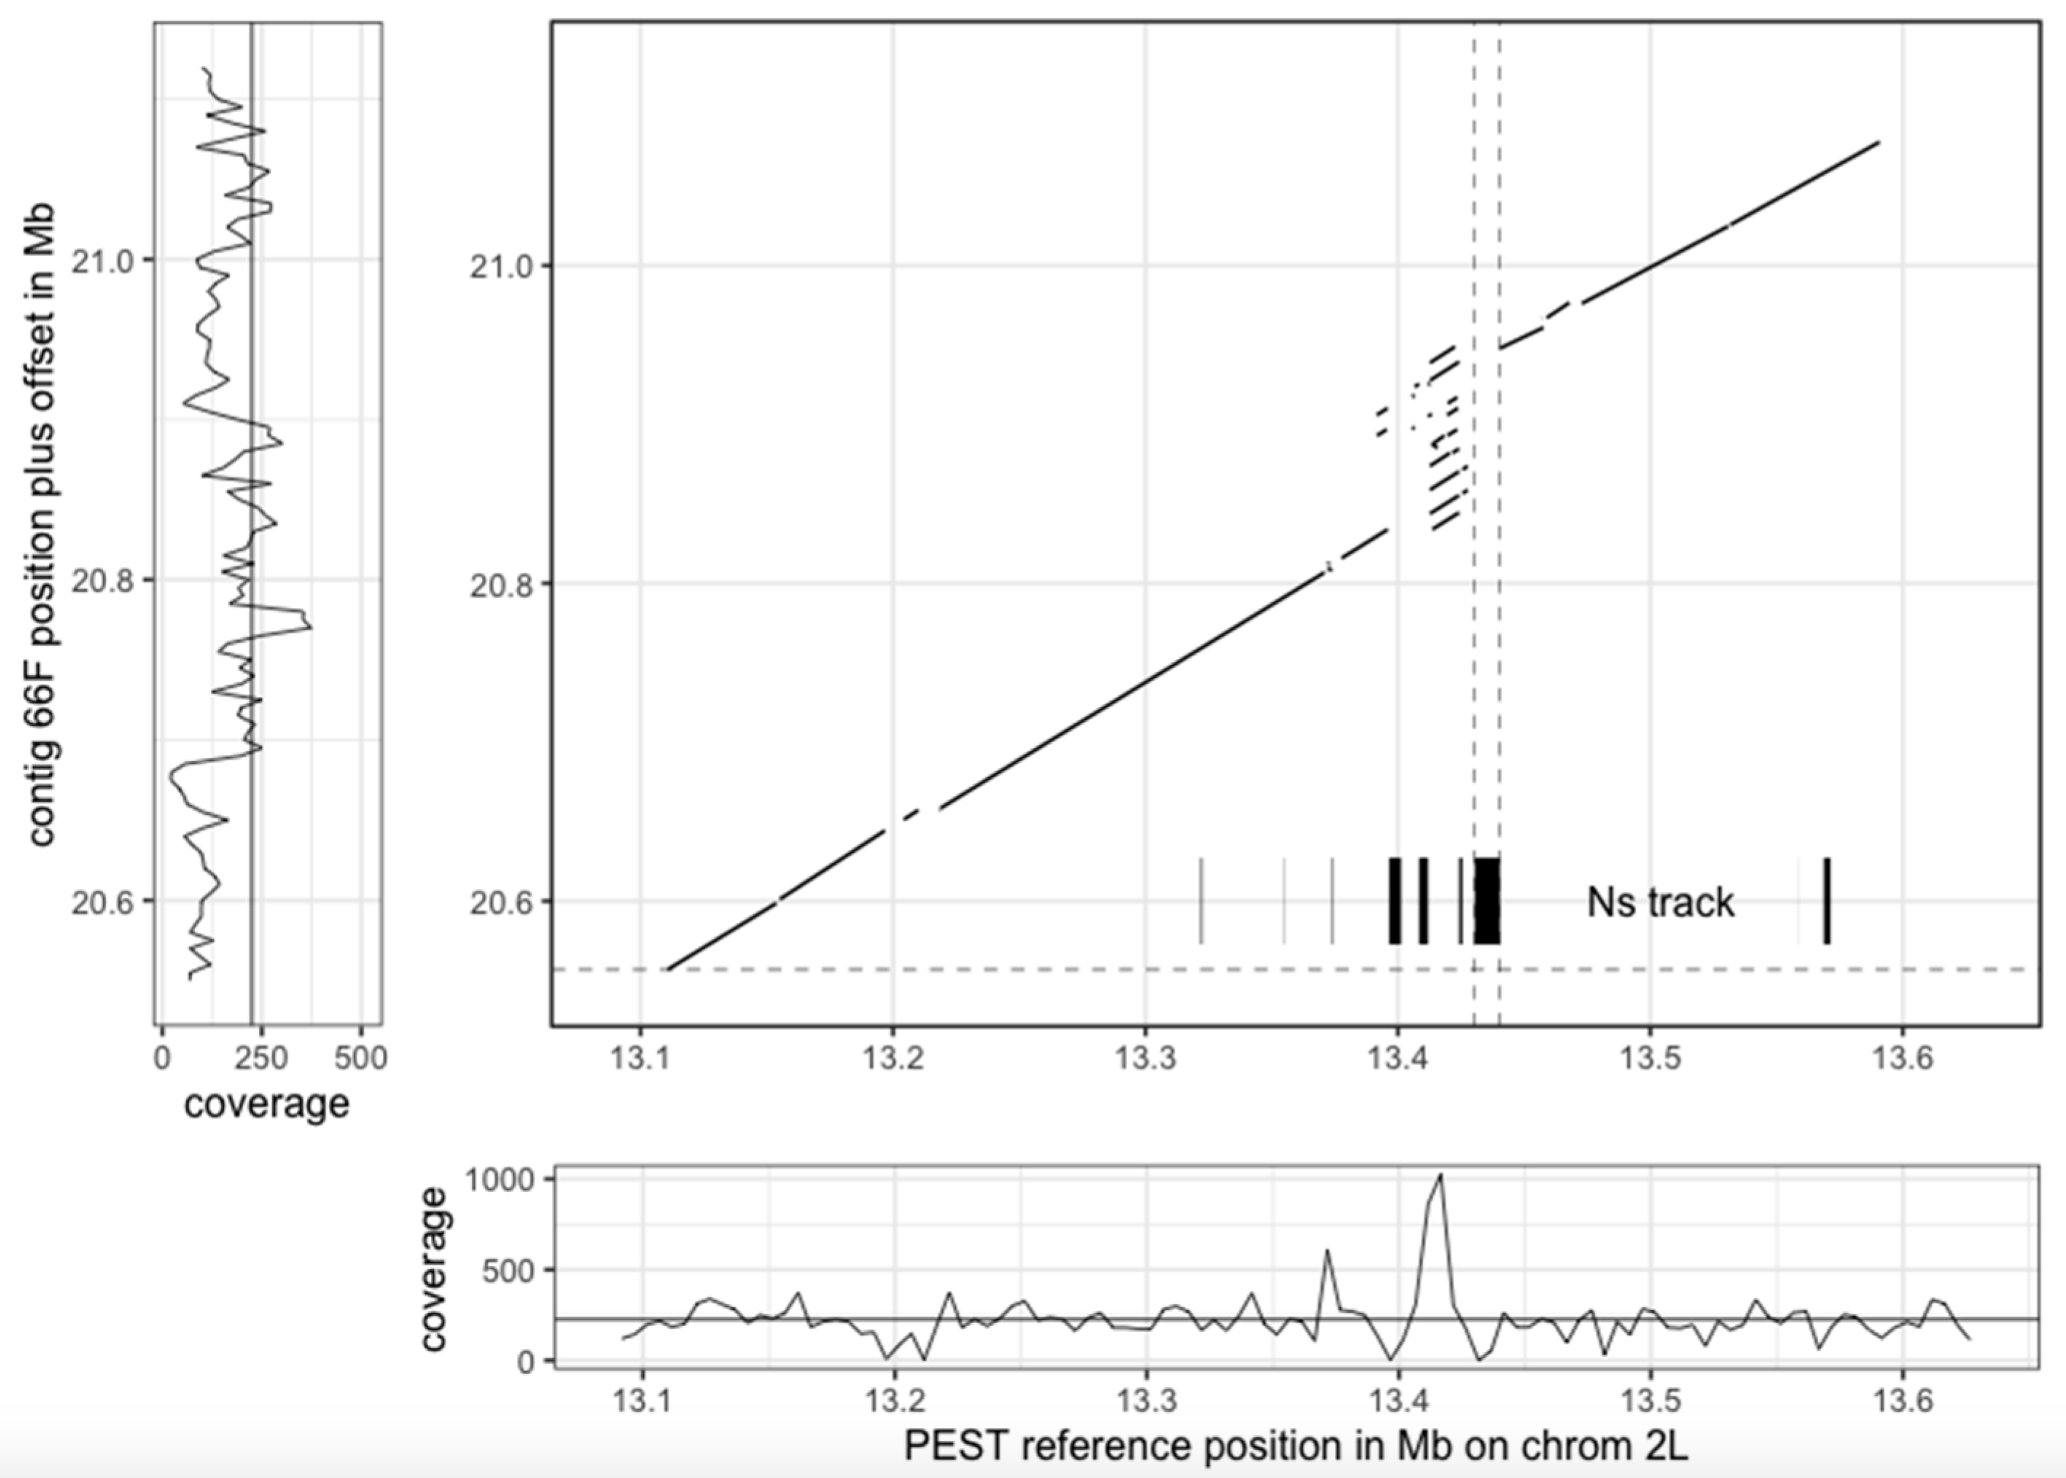
\includegraphics[width=1.0\textwidth]{repeatexpansion.png}
\floatfoot{\small{ Example of a compressed repeat in PEST that has been expanded by the PacBio assembly. Dotted vertical lines represent a gap in the PEST assembly (10,000 Ns) between scaffolds, which is now spanned by the single PacBio contig. Coverage plot of the PacBio subreads aligned to PEST (bottom) highlights the region where excess coverage indicates a collapsed repeat in PEST, in contrast the coverage of PacBio subreads aligned to the PacBio contig (left) is more uniform. }}
\end{centering}
\end{figure}

\subsection{Corrected order and orientation vs PEST scaffolding}

\par{
I also identified several potential rearrangements in the 20-22 Mb region of the X chromosome (see figure \ref{figure:x_inversion}). PEST has contig breaks at the putative breakpoints relative to the assembly, however, given that a single PacBio contig spans the full region and that potential breakpoints relative to PEST are supported by multiple reads, the most likely explanation is an order and orientation issue in PEST, perhaps combined with a potential inversion difference between \textit{Anopheles coluzzii} and the PEST reference. In addition, the contig contains a relatively large region (~380 kb in total) of PacBio sequence corresponding to several pieces in the UNKN section of PEST that can now be assigned to the X chromosome.
}

\begin{figure}[htbp!]

\caption{Resolved order and orientation error in PEST scaffolding}
\label{figure:x_inversion}
\begin{centering}
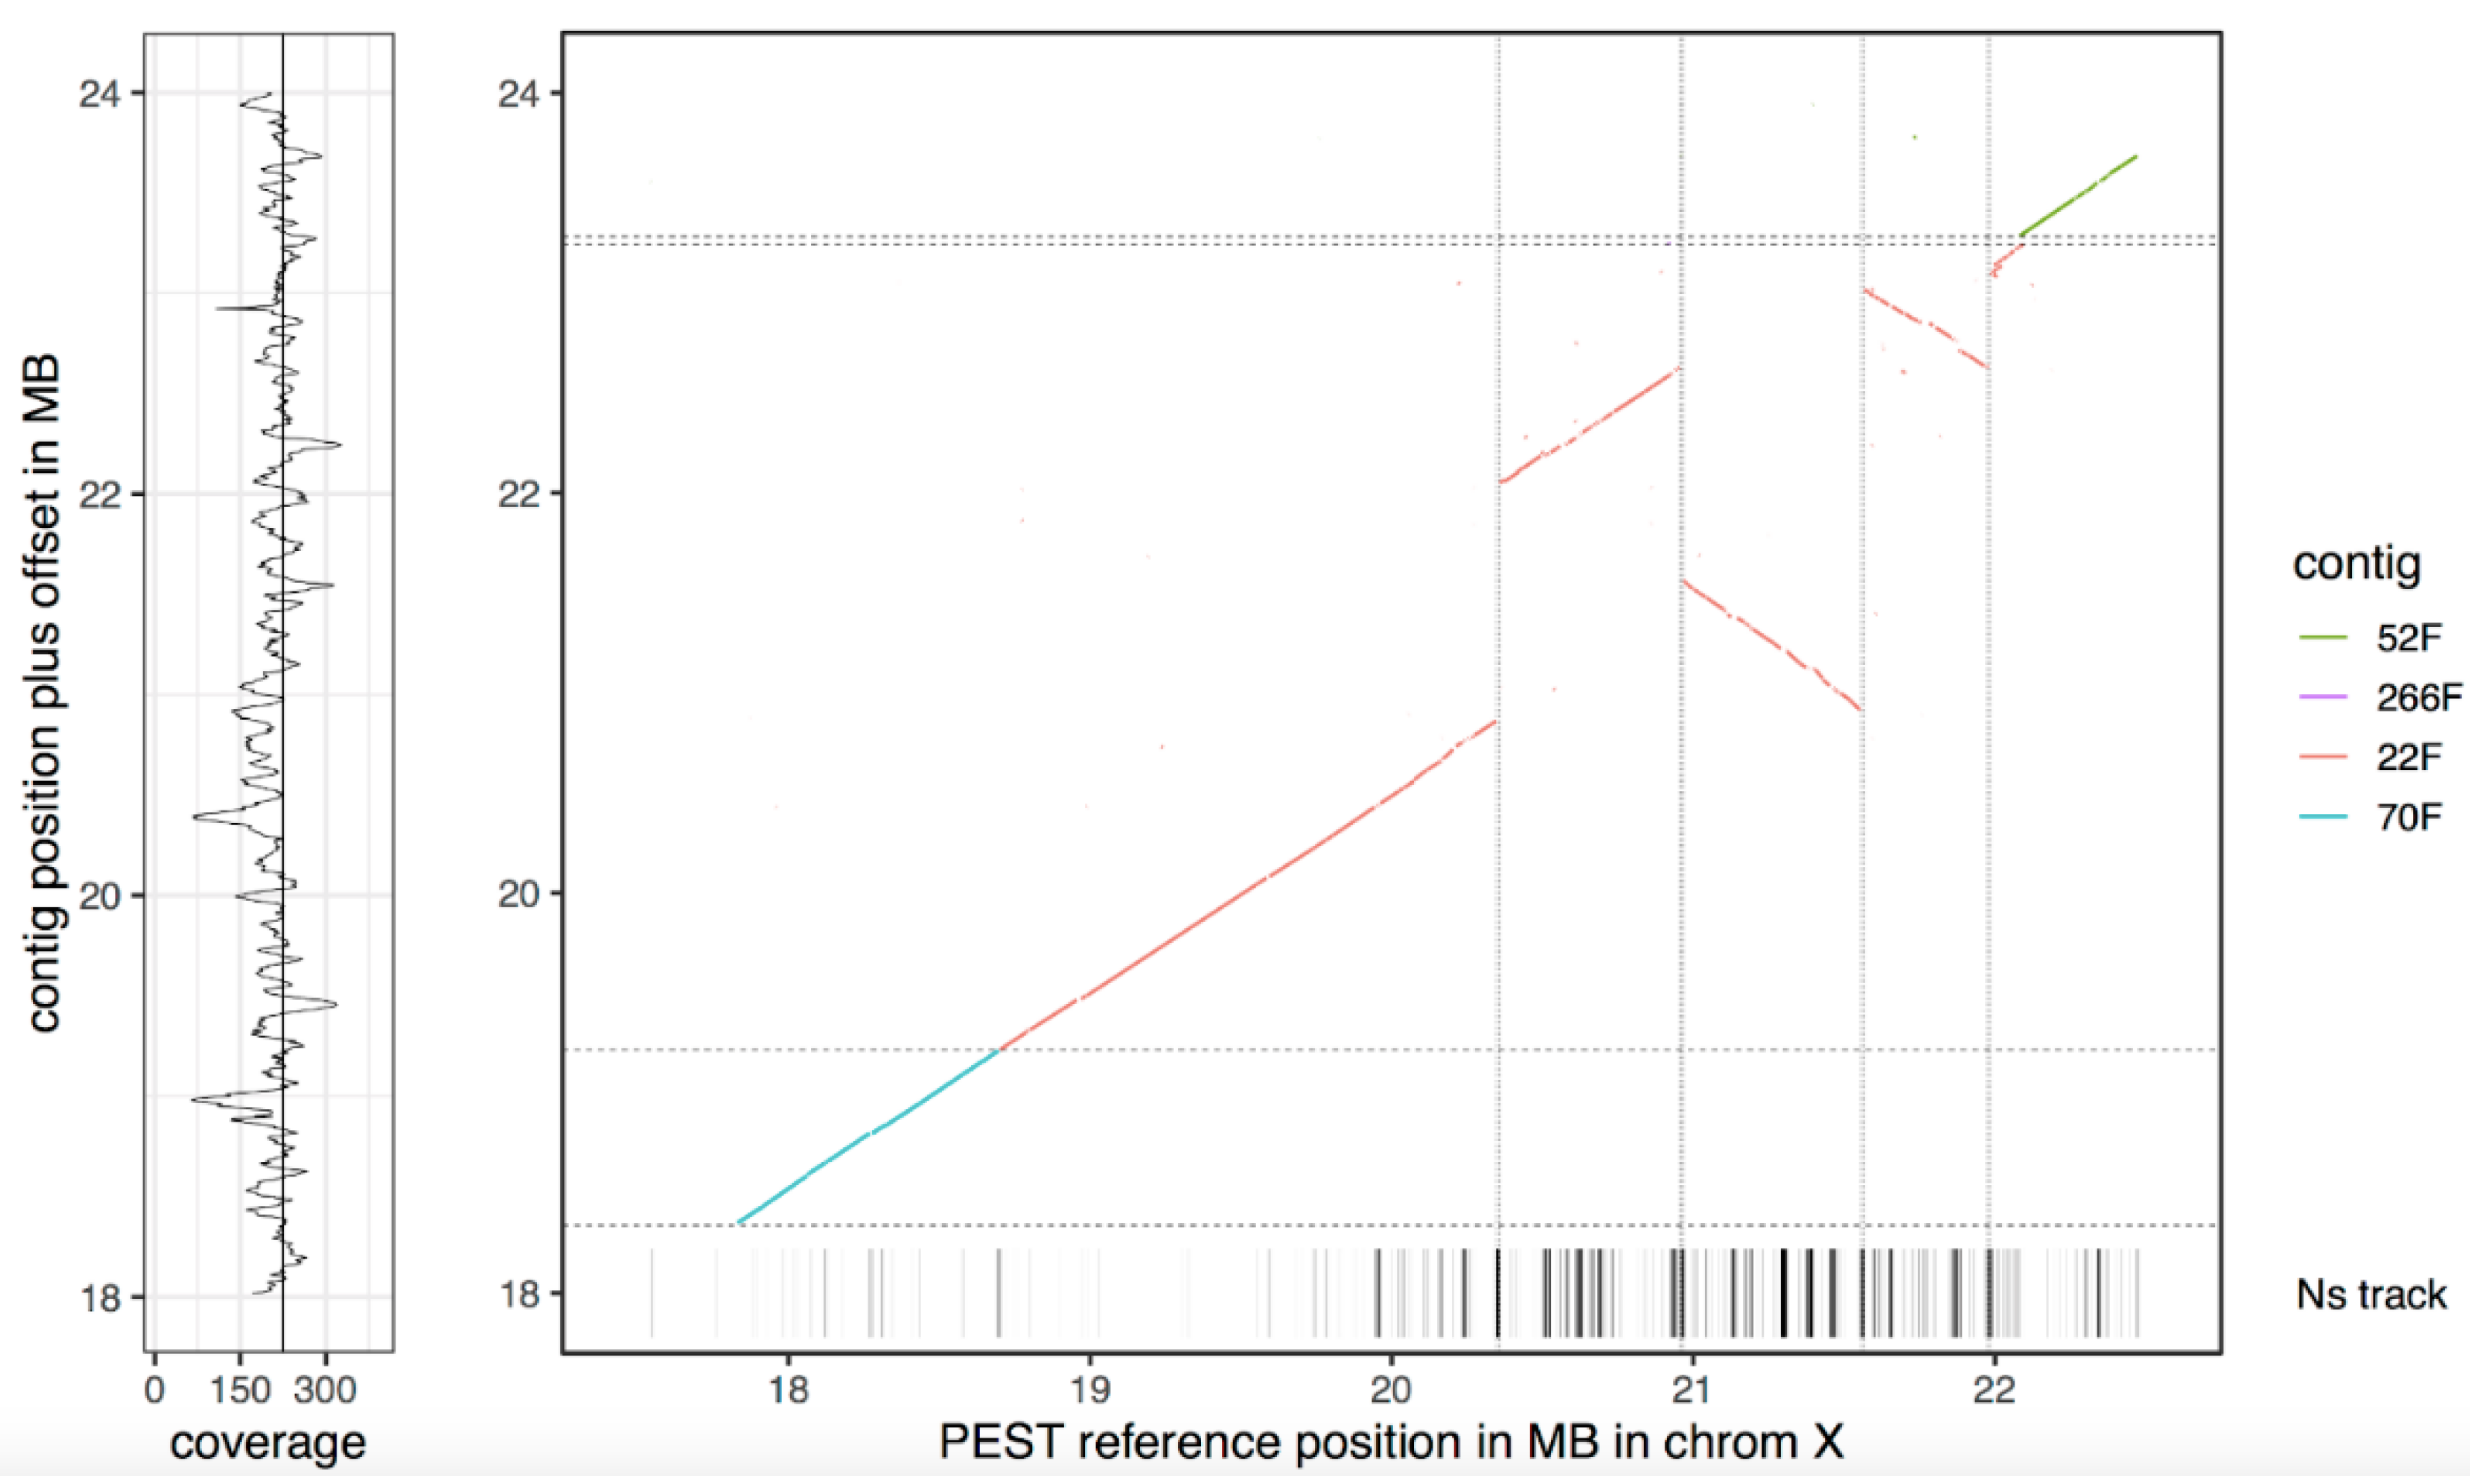
\includegraphics[width=1.0\textwidth]{x_inversion.png}
\floatfoot{\small{Alignment of X pericentromeric contigs to PEST, highlighting likely order and orientation issues in the PEST assembly that are resolved by a single PacBio contig.}}
\end{centering}
\end{figure}


\subsection{Identification of some UNKN PEST sequence as haplotigs}\label{section:unkn}

\par{
The PEST annotation also retains a large bin of unplaced contigs (27.3 Mb excluding Ns) designated as the UNKN (unknown) chromosome. Previously, I mapped either assembly contigs onto the PEST reference or subreads against the assembly. Now I show the reverse of the former and map PEST contigs onto the assembly. If an UNKN contig alignment overlaps a chromosomal contig alignment versus the assembly (both with mapping quality (mapq) 60), it is likely to be a haplotig in the UNKN (see figure \ref{figure:unknplace}). In total, I find that 7.27 Mb are haplotigs (i.e., also have high quality PEST chromosomal alignments to the same location in the assembly).
}

\begin{figure}[htbp!]

\caption{UNKN placement and haplotig identification}
\label{figure:unknplace}
\begin{centering}
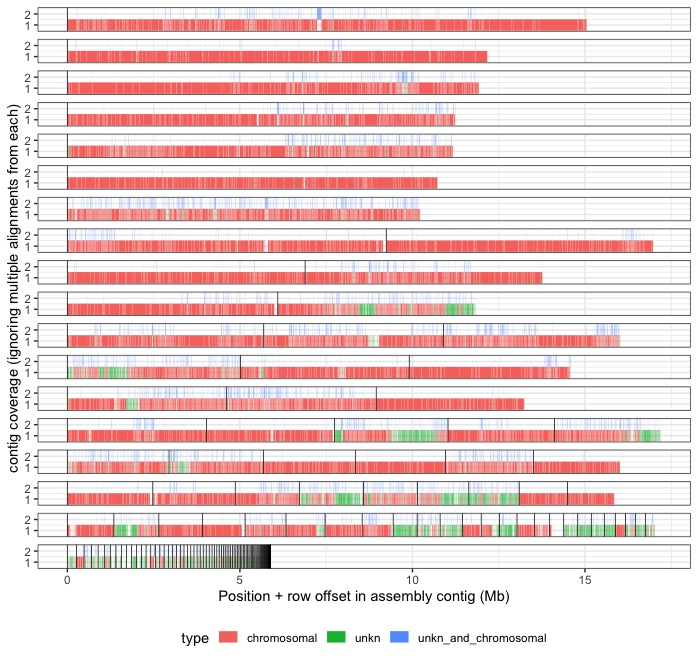
\includegraphics[width=1.0\textwidth]{Unkn_placement_haplotig.jpeg}
\floatfoot{\small{Contig coverages (ignoring multiple alignments for each chromosomal and UNKN sequence) of PEST aligned to the curated assembly showing placement of previously unplaced sequence (green on contigs that also have red (chromosomal) alignments). I also note the locations where both UNKN and chromosomal sequence align to the same location in the curated assembly which are likely haplotigs in the PEST UNKN scaffold.}}
\end{centering}
\end{figure}

\subsection{Placement of previously unplaced genes}\label{section:unkn}
\par{
In addition to the UNKN haplotig sequences, I found another 10.9 Mb of the alignments are newly placed sequence that do not overlap with PEST chromosomal alignments but are in contigs which have a large amount (>100kb) of chromosomal alignments meaning these contigs are confidently ordered and oriented in their chromosomal contexts. The UNKN bin also contains 737 annotated genes. Remarkably, our single-insect assembly now places 667 (>90\%) of these formerly unplaced genes into their appropriate chromosomal contexts (2L:148 genes; 2R:162 genes; 3L: 126 genes; 3R:91 genes; X:140 genes; unplaced:70 genes; detail on placement of specific genes can be found in the supplement of our paper\cite{singlemosquito}), which together with their flanking sequence comprise 8.9 Mb of sequence. Altogether, this means that 32.6\% of the UNKN chromosome is now placed in the genome and 26.6\% is determined to be haplotigs, along with 90\% of the genes that were contained within it. Much of the remaining sequence do not have high mapping quality subreads when aligning subreads to the PEST reference meaning they are either repeats or junk sequence.
}

\subsection{PEST contig coverage on PacBio curated assembly}

\par{
In addition to looking for the two contig coverage areas and confirming that they primarily come from haplotigs in the UNKN scaffold, other abnormalities such as zero contig coverage regions are looked for. In figure \ref{figure:reverse_coverage} there is significant zero coverage regions. However, most of these are intermittently zero and one likely just indicating sequence divergence rather than an incomplete PEST reference. There are a few more solidly zero coverage regions, but they are not dramatically long (<200Kb). Still, the BUSCO \ref{table:busco} analysis shows that there are fewer complete genes and more fragmented and missing genes in the PEST reference as compared to the PacBio assembly. These regions likely account for some of that difference.
}

\begin{figure}[htbp!]

\caption{PEST contig coverage when aligned to PacBio curated assembly}
\label{figure:reverse_coverage}
\begin{centering}
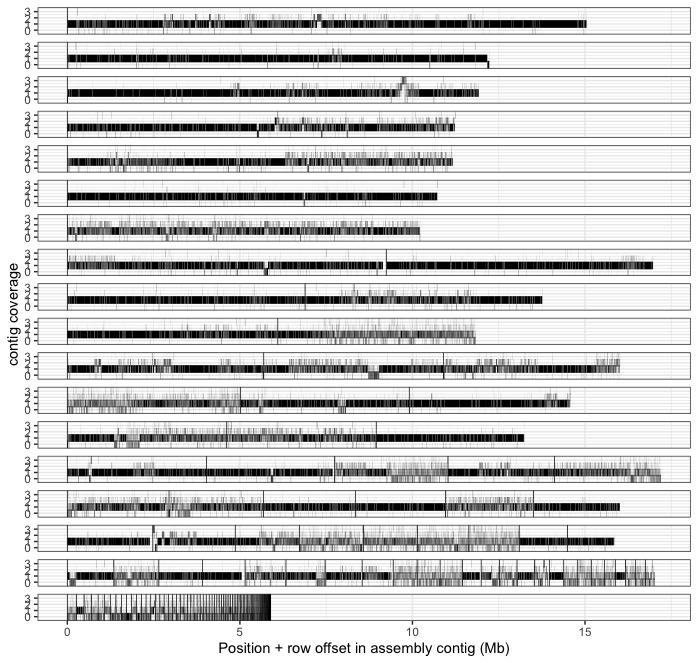
\includegraphics[width=1.0\textwidth]{Reverse_contig_coverage.jpeg}
\floatfoot{\small{Contig coverages of PEST aligned to the curated assembly. When comparing to figure \ref{figure:unknplace}, most of the two-coverage areas likely come from haplotigs in the UNKN scaffold. But there is some significant zero coverage areas as well.}}
\end{centering}
\end{figure}

\section{Discussion}

\par{
Long-read PacBio sequencing has been utilized extensively to generate high-quality eukaryote de novo genome assemblies, but because of the relatively large DNA input requirements, it has not been used to its full potential for small organisms, requiring time-consuming inbreeding or pooling strategies to generate enough DNA for library preparation and sequencing. Here we present, to our knowledge, the first example of a high-quality de novo assembly from a single insect. This assembly, using only one individual and one sequencing technology, exhibits a higher level of contiguity, completeness, accuracy, and degree of haplotype separation than any previous Anopheles assembly, demonstrating the impact of long reads on assembly statistics. While the assembly did not achieve independent full chromosomal scale assignment of contigs, its mega-base scale contiguity without gaps immediately provides insights into gene structure and larger-scale genomic architecture, such as promoters, enhancers, repeat elements, large-scale structural variation relative to other species, resolution of tandem repeats (figure \ref{figure:x_inversion}), and many other aspects relative to functional and comparative genomics questions.
} 
\par{
About a third of the genome for this diploid individual is haplotype-resolved and represented as two separate sequences for the two alleles, thereby providing additional information about the extent and structure of heterozygosity that was not available in previous assemblies, which have been constructed from many pooled individuals. In contrast with approaches requiring multiple individuals, the ability to generate high-quality genomes from single individuals greatly simplifies the assembly process and interpretation, and will allow far clearer lineage and evolutionary conclusions from the sequencing of members of different populations and species. Further, if parental samples are available, the recently developed trio binning assembly approach \cite{triobinning} can be used to further segregate alleles for a full haplotype-resolved assembly of both parental copies of the diploid offspring organism.
} 
\par{
The assembly presented here provides an excellent foundation towards generating an improved chromosome-scale reference genome, using the previous PEST reference, scaffolding information from genetic maps, technologies such as Hi-C (e.g., \cite{falconphase}), or alignment of the contigs to closely related species' references. These approaches can also be used to highlight areas of potential improvements to the FALCON-Unzip assembler and to Purge Haplotigs, or other packages used to identify haplotypic contigs. As one example, we noticed in the context of the incomplete haplotype purging described above that some neighboring contig ends exhibited overlaps relative to the PEST reference (figure \ref{figure:haplotig}). The interpretation of such haplotype contig overlaps was corroborated by the observed halving of average sequencing depth over the regions of overlap. These methods could incorporate adjustments to try to account for haplotypic regions in the ends of contigs rather than complete contigs being fully haplotypic.
} 

\par{
We noted the importance of the initial DNA size distribution in conjunction with this protocol. Since neither shearing prior to library construction nor size-selection thereafter were employed, the starting high-molecular weight DNA should contain fragments at greater than ~20 kb on average, and without the significant presence of short (smaller than $\approx$5 kb) DNA fragments. Further research into suitable DNA extraction, storage and transportation methodologies is needed to fulfill these requirements for a broader spectrum of different species and environments, in order to allow for the preparation of suitable DNA samples from wild-caught samples originating in sometimes remote areas with limited sample preparation infrastructure.
} 

\par{
The new workflow described here has now become standard procedure for creating high quality reference genomes for small organisms. And the more recent advent of HiFi data has made even higher quality genome assemblies of insects and other small organisms routine. This represents an important prerequisite in view of large-scale initiatives such as i5K and the Earth BioGenome Project \cite{EBGP}\cite{arthropoddiversity}. In addition, other research areas with typically low DNA input regimes can benefit from the described new workflow, e.g., metagenomic community characterizations of small biofilms, DNA isolated from needle biopsy samples, minimization of amplification cycles for targeted or single-cell sequencing applications, and others.
}


